\documentclass[10pt,twocolumn]{article}
\usepackage[margin=0.8in]{geometry}
\usepackage[T1]{fontenc}
\usepackage{amsmath}
\usepackage{newtxtext,newtxmath}  % after amsmath; provides the amssymb symbols
\setmonofont[Scale=MatchLowercase,BoldFont=Inconsolatazi4-Bold.otf]{Inconsolatazi4-Regular.otf}  % XeTeX (tectonic): newtxtext uses fontspec, so the mono font must too
\usepackage{booktabs}
\usepackage{graphicx}
\usepackage{tikz}
\usetikzlibrary{positioning,arrows.meta}
\usepackage[hidelinks]{hyperref}


\title{Team \texttt{ByeByeHelloHaHaHa}: A Generic, Render-Light Pipeline for\\4D Human--Object Reconstruction from a Single Video\\[2pt]
\large V2D Challenge 2026, Track 1 (Reconstruction) --- Technical Report}
\author{Hao-Yu Chan\\University of Michigan}
\date{}

\begin{document}
\maketitle

\begin{abstract}
I reconstruct, from one static third-person RGB video and nothing else, an MHR human sequence and a textureless
object mesh with a per-frame similarity pose. Every clip goes through the same stages with the same settings: a
vision-language model names the object, SAM~3 tracks the actor and the object, MoGe-2 and OpenD4RT give metric,
temporally consistent depth, SAM~3D Body gives the human, and SAM~3D Objects gives the object mesh together with a
pose-and-scale \emph{layout} that I use as extra starting hypotheses for a render-free point fit. A contact-, floor-
and penetration-aware joint placement and a final smoothing stage tuned to the acceleration metrics complete the
pipeline. My reference run scores CD-H 14.24\,cm, CD-O 26.93\,cm, ACC-H 0.1375, ACC-O 0.0732 and PEN 0.0015\,cm
on the public leaderboards. I report the ablations that shaped it, including a render-and-compare variant that
trades ACC-O for CD-O.
\end{abstract}

\section{Task and metrics}
Track~1 provides 30 clips (10 objects, 3 clips each; 1536$\times$1152, 30\,fps, 16{,}563 frames of which 9{,}877 are
scored) from a static camera, with no intrinsics, no object template and no depth. A submission is, per clip, MHR
parameters (pose, scales, shape) for the actor and an object mesh ($\le$4{,}096 faces after packing) with a
rotation, translation and scale per frame. The scorer aligns the prediction once, by a Sim(3) on the human at the
first scored frame, then reports five metrics, each a separate leaderboard and each a mean over clips: Chamfer
distance of the human (CD-H) and the object (CD-O), acceleration error of 22 human joints (ACC-H) and of the
object translation (ACC-O), and the penetration depth of 512 hand points into the object (PEN). The final ranking
sums the five ranks.

Two properties of the metrics guided my design. (i) Because alignment happens once, any drift in scale or depth
after the first scored frame is never forgiven. (ii) ACC-O uses only the object translation, i.e.\ the path of the
mesh origin, and a zero-acceleration prediction scores exactly the mean ground-truth acceleration ($\approx$0.074 on
the leaderboard). A noisy track is therefore worse than a static one, and the mesh origin should be the object's centre.

\section{Pipeline}
Figure~\ref{fig:pipe} shows the stages. A single driver (\texttt{scripts/e2e\_vm.py}) runs them on one Colab GPU VM;
stages resume from their outputs, and nothing in them depends on which object a clip shows.

\begin{figure}[t]
\centering
\scriptsize
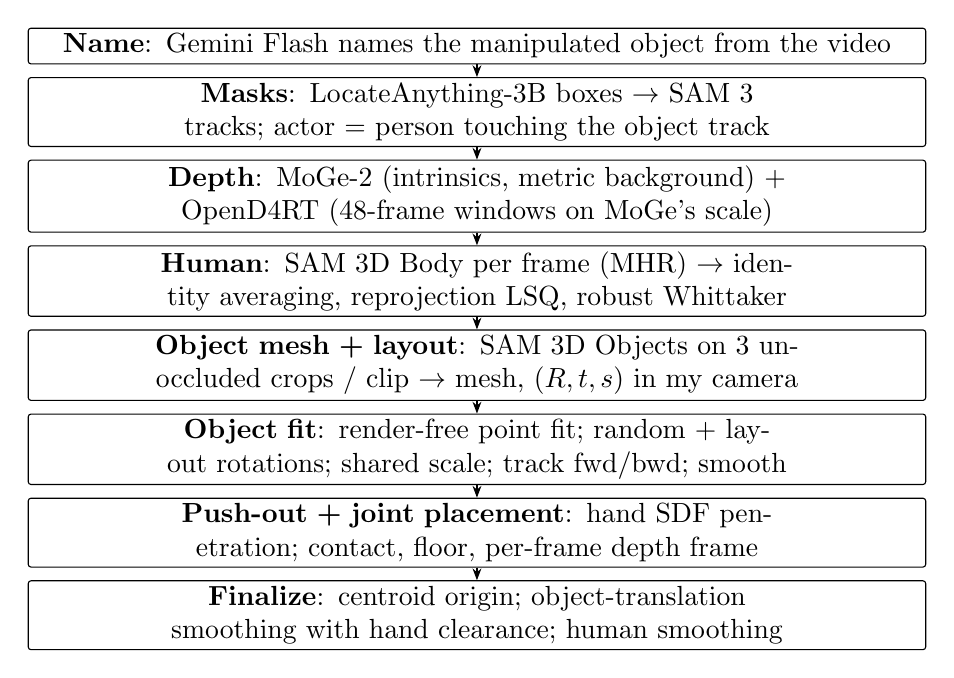
\begin{tikzpicture}[node distance=1.6mm, box/.style={draw, rounded corners=1pt, align=center, inner sep=2pt,
  minimum width=0.94\columnwidth, text width=0.92\columnwidth}, >={Stealth[length=1.5mm]}]
\node[box] (n) {\textbf{Name}: Gemini Flash names the manipulated object from the video};
\node[box, below=of n] (m) {\textbf{Masks}: LocateAnything-3B boxes $\to$ SAM~3 tracks; actor = person touching the object track};
\node[box, below=of m] (d) {\textbf{Depth}: MoGe-2 (intrinsics, metric background) + OpenD4RT (48-frame windows on MoGe's scale)};
\node[box, below=of d] (h) {\textbf{Human}: SAM~3D Body per frame (MHR) $\to$ identity averaging, reprojection LSQ, robust Whittaker};
\node[box, below=of h] (o) {\textbf{Object mesh + layout}: SAM~3D Objects on 3 unoccluded crops / clip $\to$ mesh, $(R,t,s)$ in my camera};
\node[box, below=of o] (f) {\textbf{Object fit}: render-free point fit; random + layout rotations; shared scale; track fwd/bwd; smooth};
\node[box, below=of f] (p) {\textbf{Push-out + joint placement}: hand SDF penetration; contact, floor, per-frame depth frame};
\node[box, below=of p] (z) {\textbf{Finalize}: centroid origin; object-translation smoothing with hand clearance; human smoothing};
\foreach \a/\b in {n/m, m/d, d/h, h/o, o/f, f/p, p/z} \draw[->] (\a) -- (\b);
\end{tikzpicture}
\caption{Track~1 pipeline (reference run \texttt{lay\_jfin}). All stages run with fixed, object-independent settings.}
\label{fig:pipe}
\end{figure}

\subsection{Object name and masks}
Gemini Flash is asked which object the person interacts with; the short answer is the only object-specific input.
LocateAnything-3B grounds the name on $\sim$11 keyframes, and the boxes seed SAM~3 video tracks, which the boxes
then vote on (moving tracks win over still ones, so a table the hand rests on is not chosen). The actor is the
foreground person whose mask touches the object track, in the image and in depth, on most scored frames. If no
track passes a coverage and motion check, a motion-seeded or depth-foreground fallback is used.

\subsection{Depth and camera}
MoGe-2 runs per frame; one field of view per clip (the median of free estimates on 16 frames) gives the
intrinsics, and the static background, a median over the clip, gives a metric reference. OpenD4RT produces
temporally consistent depth in 48-frame windows (overlap 16); each window is scaled to the MoGe background on
static pixels, windows are blended, and each frame is stabilized against the background. The camera is static, which
gives a check on OpenD4RT: its camera extrinsics should be the identity, and they nearly are. A Sim(3) fitted on
background points from each frame to its window's first frame has a median rotation of 0.12$^\circ$ and a median
translation of 0.2\% of the scene depth over the 30 clips (worst 0.63$^\circ$ and 1.2\%), which supports
OpenD4RT's geometry as a reliable depth source. A floor plane is fitted
for the joint stage.

\subsection{Human}
SAM~3D Body runs per frame on the actor box and mask with my intrinsics and returns native MHR parameters.
Post-processing fixes one identity (mean scales and shape over fully visible frames), re-solves each translation so the
22 scored joints reproject where SAM~3D Body put them, and applies a robust Whittaker smoother (second differences)
to translation, root rotation and pose, down-weighting and re-solving outlier frames. I keep SAM~3D Body's own
depth for the body: moving it along the ray to the depth map cost 2\,cm CD-H (Table~\ref{tab:abl}). The body then
defines the metric frame: the ratio of depth-map to body depth over the actor mask rescales the depth used for
the object.

\subsection{Object mesh and layout}
Three crops per clip are taken from the best unoccluded frames (large mask, little outline shared with the actor,
$\ge$30 frames apart). For each, SAM~3D Objects receives the full frame, the full-resolution mask and a pointmap
from my depth at the body's scale, and returns a mesh and a layout $x_\text{cam} = s R v + t$ in my camera.
Meshes are cleaned (floaters removed, main part kept), normalized to unit size and decimated to $\le$4{,}000 faces.
The layout is re-expressed for the normalized mesh.

\subsection{Object pose fit}
The pose model is $x_\text{cam} = s R p + t$ for points $p$ sampled on the mesh; no rasterizer is used. Four robust
(Geman--McClure) terms compare it with the observations: model points falling outside the object $\cup$ actor
mask (occlusion by the actor is free), object-mask pixels not covered by projected points, interior object depth
to the nearest model point, and front-facing model points against the depth map. Per clip I (1) screen each
candidate mesh from many rotations on a few well-visible keyframes, adding each SAM~3D layout from that mesh as a
start (and its 25$^\circ$ perturbations) on its own frame; (2) fix one scale, the weighted median of keyframe
scales; (3) track forward and backward from the best keyframe, each frame starting from the previous pose and six
rotations of it, with a rotation-jump penalty; and (4) refine all frames jointly with second-difference
penalties on $t$ and $R$.

\subsection{Penetration push-out and joint placement}
The packed mesh is turned into a signed-distance grid with the scorer's inside rule (generalized winding numbers).
A refit adds a hinge on the signed distance of every hand vertex the MHR finger parameters move, keeping the data
terms so the object stays where the video puts it. The joint stage then places the object relative to the body:
a per-frame depth ratio between the depth map and the rendered body (smoothed) defines one consistent depth
frame; contact candidates are hand and sole points projecting onto the object mask; a search along the camera
ray ($s \to a s$, $t \to a t$, which leaves the image unchanged) trades depth agreement, contact, floor and a
scale prior; a ray-only per-frame refinement follows, and discrete rotation hypotheses resolve poses the image
cannot separate (e.g.\ a ring's two tilts).

\subsection{Finalization}
The mesh origin is moved to the surface centroid (the pose compensates, so the surface is unchanged), so that
ACC-O follows the object's centre. The object translation is then re-solved as
$\arg\min_t \|t - t_0\|^2 + \lambda_o \|D_2 t\|^2 + w \sum \mathrm{relu}(m - \mathrm{SDF}(\text{hand}))^2$ with
$\lambda_o = 10^5$, rotation and scale kept, and the human receives one more Whittaker pass
($\lambda_{t,r,p} = 1000, 600, 600$).

\section{Results}
Table~\ref{tab:main} gives the reference run. Each leaderboard ranks my best submission on it separately; the
reference run is the single pipeline I describe and reproduce.

\begin{table}[t]
\centering\small
\setlength{\tabcolsep}{3pt}
\begin{tabular}{lccccc}
\toprule
run & CD-H & CD-O & ACC-H & ACC-O & PEN \\
\midrule
\texttt{lay\_jfin} (mine) & 14.24 & 26.93 & 0.1375 & 0.0732 & 0.0015 \\
\bottomrule
\end{tabular}
\caption{Public leaderboard scores of the reference run (cm; lower is better).}
\label{tab:main}
\end{table}

\paragraph{Ablations.} Table~\ref{tab:abl} lists leaderboard results of the variants that led to the reference
run. Rows marked with a dash were submitted to a subset of boards only.

\begin{table*}[t]
\centering\small
\setlength{\tabcolsep}{5pt}
\begin{tabular}{llccccc}
\toprule
& variant & CD-H & CD-O & ACC-H & ACC-O & PEN \\
\midrule
A & generic pipeline, Hunyuan3D-2.1 meshes, no finalization (\texttt{e2e\_box}) & 14.20 & 33.34 & 0.170 & 0.119 & 0.00091 \\
B & A + finalization, $\lambda_o = 10^3$, no human smoothing & 14.20 & 33.25 & 0.170 & 0.0876 & 0.00089 \\
C & A + finalization, $\lambda_o = 10^4$ & -- & -- & -- & 0.0749 & -- \\
D & C + object follows the holding wrists' acceleration & -- & -- & -- & 0.0848 & -- \\
E & B + human Whittaker $(10^3, 200, 200)$ & 14.27 & -- & 0.1374 & -- & -- \\
F & body depth moved along the ray to the D4RT actor depth & 16.16 & -- & 0.172 & -- & -- \\
G & A + render-and-compare refinement + finalization & -- & 30.30 & -- & -- & -- \\
\midrule
H & SAM~3D web-demo meshes (RGB only), no layout seeds & -- & 28.63 & -- & -- & -- \\
I & H + render-and-compare + finalization (\texttt{s3dall\_rf\_fin}) & 14.24 & \textbf{24.48} & 0.1375 & 0.0748 & 0.00126 \\
J & SAM~3D on my crops + layout seeds (\texttt{lay\_jfin}, reference) & 14.24 & 26.93 & 0.1375 & \textbf{0.0732} & 0.00148 \\
K & J + render-and-compare & 14.24 & 26.63 & 0.1375 & 0.0749 & \textbf{0.00084} \\
L & web-demo meshes + layout seeds transferred by ICP & 14.24 & 28.52 & 0.1375 & 0.0737 & 0.00264 \\
M & L + render-and-compare & 14.24 & 26.37 & 0.1375 & 0.0746 & 0.00105 \\
\bottomrule
\end{tabular}
\caption{Leaderboard ablations (cm). A--G use Hunyuan3D-2.1 meshes; H--M use SAM~3D Objects meshes. Final runs
(I--M) use $\lambda_o = 10^5$ and human smoothing $(1000, 600, 600)$.}
\label{tab:abl}
\end{table*}

\paragraph{What mattered.}
\emph{Object meshes} were the largest CD-O lever: replacing Hunyuan3D-2.1 by SAM~3D Objects moved CD-O from
33.3 to 28.6\,cm without any other change (A vs.\ H).
\emph{Acceleration-aware finalization} took ACC-O from 0.119 to 0.073--0.075, i.e.\ to the level of a static
object, for no measurable CD-O cost (A--C); coupling the object to the wrists hurt (D vs.\ C), since per-frame wrist
estimates are noisier than the object's true motion.
\emph{Human smoothing} brought ACC-H from 0.170 to 0.137 for $+0.04$--$0.07$\,cm CD-H (E, I--M); moving the body to
the depth map hurt CD-H by 2\,cm (F), so the body, not the depth map, defines the metric frame.
\emph{Render-and-compare refinement} (nvdiffrast, masks only, with an occlusion rule against the rendered body)
helps CD-O on top of a render-free fit (G: $-3$\,cm; I vs.\ H: $-4.1$\,cm) but slightly roughens the object track
(ACC-O $+0.002$, J vs.\ K), which is why the reference run omits it.
\emph{Layout seeds} gave the best ACC-O (J) but not the best CD-O: with the same web-demo meshes, adding the seeds
cost $\approx$2\,cm CD-O (I vs.\ M), while the mesh source mattered little once seeds were used (K vs.\ M).

\paragraph{Reference run choice.}
Variant I has the best CD-O and J the best ACC-O; their summed ranks over the three object boards are within two
places. I report J because it is fully automatic: variant I relies on meshes generated interactively in the SAM~3D web
demo, which a single-command reproduction cannot rerun. In the web demo I selected the object so that its
mask matched my SAM~3 mask, so in principle running SAM~3D Objects locally on the same frame and mask, from RGB
only as the demo does, should reproduce those meshes and make variant I automatic as well; I had no compute units left to
verify this.

\section{Failure cases and limitations}
I picked the failures from per-clip proxy metrics of the reference run (object mask IoU and depth error against
my own masks and depth, since the leaderboard reports only means). Three clips stand out; Figure~\ref{fig:fail}
shows each in the input view and from a side camera.

\emph{Thin ring without depth (clip 1, hula hoop; object IoU 0.19).} The depth map does not resolve a 5\,cm
tube, so only 7 of 341 frames give object depth and the image fixes the hoop only up to a scale along the ray. The
joint stage then sets that scale from hand contact alone and shrinks the hoop by 24\%, from the 0.90\,m of the image fit to 0.69\,m (the image fits of the other two hoop
clips give 0.84\,m), which pulls it toward the camera: the leg goes through the hoop in the video
but passes beside it in the reconstruction.

\emph{Object occluded in every crop (clip 2, hula hoop; IoU 0.41).} The hoop is spun around the body, so all three
crops show a ring cut by the torso. SAM~3D Objects reconstructs from these partial rings and its layouts fall
largely outside the mask (35--43\% of their points inside, against 74--100\% for the other two hoop clips); the fit
loss is ten times that of clip~0. The resulting track keeps the ring's outline in the image but places it upright
through the torso, which no term rejects, since penetration is only checked for hand points.

\emph{Flat object seen edge-on (clip 14, tablet; IoU 0.42).} The tablet lies on a table nearly in line with the
camera, so its mask is a thin sliver. The three SAM~3D layouts disagree on its size by a factor of 2.5
(0.18--0.45\,m), the joint stage switches between rotation hypotheses, and in the unheld frames the tablet sits near
the floor in front of the table instead of on it.

\begin{figure*}[t]
\centering
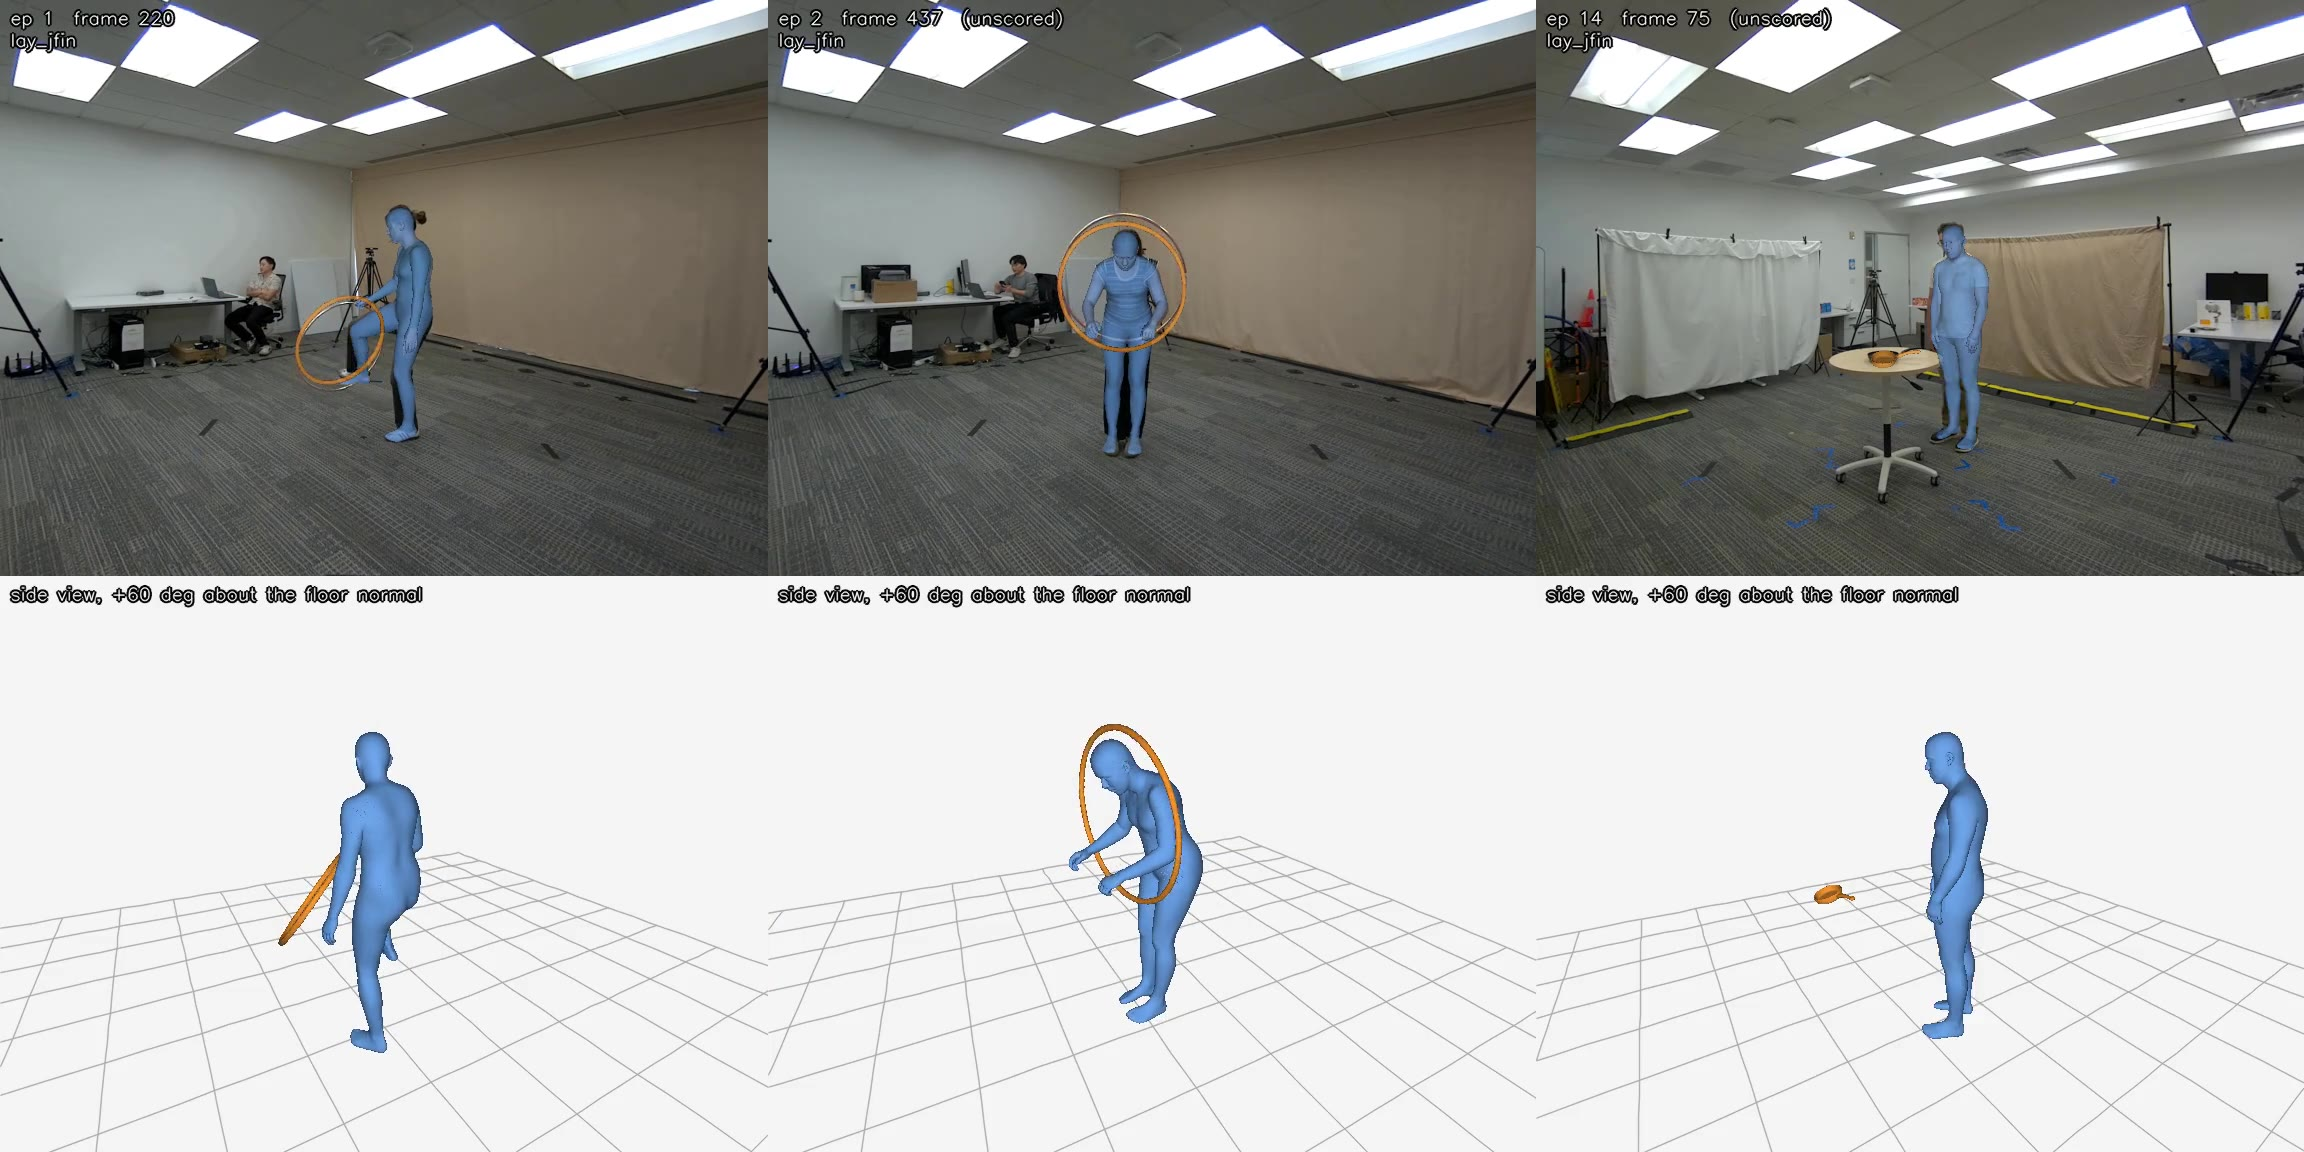
\includegraphics[width=\textwidth]{figs/failure_cases.jpg}
\caption{Failure cases of the reference run (human blue, object orange). Top: input frame with the reconstruction;
bottom: side view, 60$^\circ$ about the floor normal. Left: clip 1, the hoop, shrunk by 24\% in the joint stage, hangs
beside the leg that goes through it in the video. Middle: clip 2, the ring is placed upright through the torso. Right:
clip 14, the tablet is placed near the floor instead of on the table.}
\label{fig:fail}
\end{figure*}

More generally, the fit has no appearance term, so symmetric or thin objects can keep a wrong rotation that the masks cannot
reject; the joint stage's discrete hypotheses only cover known ambiguities. Object scale comes from a single depth
frame tied to the body, so a biased body depth biases the object. A noisy object track is clipped toward static by
the finalization, which helps ACC-O but cannot recover true fast motion.

I see depth resolution as the main limit of the current approach. OpenD4RT, the open reimplementation of D4RT I
use, takes 256$\times$256 inputs, i.e.\ the 1536$\times$1152 frame downsampled about 6$\times$ horizontally, so thin
and small objects cover only a few depth samples: the hoop's tube in clip~1 is one example, and the edge-on tablet
in clip~14 another. I did not have access to the original D4RT weights; with them I would expect better object
depth on such objects, and with it better object placement and CD-O.

\section{Compute and reproduction}
All model inference ran on Google Colab (L4 at 1.54 and A100 at 5.3 compute units per hour); the laptop (6\,GB GPU) ran
only orchestration, light geometry and the render-and-compare variants. SAM~3D Objects takes 13--40\,s per crop on an A100 (90 crops); the
object to joint stages for 30 clips take about 3\,h on one L4, and finalization a few minutes.

Code: \url{https://github.com/ChanHaoHao/4DHumanObjectInteraction}, commit \texttt{ea90fbc} (branch \texttt{e2e-box}). On a Colab A100 session (\texttt{colab new -s e2e -{}-gpu A100}), one command runs every stage
for all 30 clips and pulls the results to \texttt{results/lay/episodes}:
\texttt{python3 scripts/e2e\_colab.py run e2e -{}-run lay -{}-episodes 0-29 -{}-sam3d}.
External models: Gemini Flash, LocateAnything-3B, SAM~3, MoGe-2, OpenD4RT, SAM~3D Body, SAM~3D Objects; no
training.

\end{document}
